\section{分布变化的局部尺度}
\label{sec:igeo-local-scale}

Fisher信息是从得分的二阶矩定义的，它是否真的衡量了“分布变了多少”？章首的均值位移给出一个线索。由第~\ref{chap:distribution-comparison}章两个等方差高斯分布的KL公式，
\[
  D_{\mathrm{KL}}\bigl(\mathcal{N}(\mu,\sigma^{2})\Vert\mathcal{N}(\mu+\delta,\sigma^{2})\bigr)=\frac{\delta^{2}}{2\sigma^{2}}=\frac12\,G_{\mu\mu}\,\delta^{2},
\]
其中$G_{\mu\mu}=1/\sigma^{2}$是式~\eqref{eq:igeo-gauss-fisher}的第一个对角元。$\delta=0.5$时，$\sigma=0.5$与$\sigma=2$分别给出$0.5$与$1/32$，正是章首的两个数。这一节先证明在一般的正则族中，邻近分布间的KL散度在二阶意义下都是$\frac12\bm{\delta}^{\top}\bm{G}\bm{\delta}$；再换参数坐标，看矩阵怎样变，它所表示的局部变化又是否保持。

\subsection{KL的二阶展开}
\label{sec:igeo-kl-expansion}

展开$D_{\mathrm{KL}}(P_{\bm{\theta}}\Vert P_{\bm{\theta}+\bm{\delta}})$，就是对$\ln p_{\bm{\theta}+\bm{\delta}}(x)$在$\bm{\theta}$处作Taylor展开再取期望。一阶项的期望是得分的期望，为零；二阶项的期望涉及对数密度的Hessian矩阵。先把这个期望与Fisher信息联系起来。

\begin{lemma}[信息等式]
\label{lem:igeo-information-identity}
设分布族正则，对每个$x\in S$，$\bm{\theta}\mapsto p_{\bm{\theta}}(x)$二阶连续可微；在给定的$\bm{\theta}$处，$\int_{S}\lVert\nabla_{\bm{\theta}}^{2}p_{\bm{\theta}}\rVert\,\mathrm{d}\nu<\infty$，$\bm{G}(\bm{\theta})$有限，并且二阶导数也可以与积分交换：
\begin{equation}
  \int_{S}\nabla_{\bm{\theta}}^{2}p_{\bm{\theta}}\,\mathrm{d}\nu=\nabla_{\bm{\theta}}^{2}\int_{S}p_{\bm{\theta}}\,\mathrm{d}\nu=\bm{0}.
  \label{eq:igeo-second-exchange}
\end{equation}
则
\begin{equation}
  \mathbb{E}_{\bm{\theta}}\bigl[\nabla_{\bm{\theta}}^{2}\ln p_{\bm{\theta}}(X)\bigr]=-\bm{G}(\bm{\theta}).
  \label{eq:igeo-information-identity}
\end{equation}
\end{lemma}

\begin{proof}
在$S$上对式~\eqref{eq:igeo-score}的商再求一次导数，商的求导法则给出
\[
  \nabla_{\bm{\theta}}^{2}\ln p_{\bm{\theta}}=\frac{\nabla_{\bm{\theta}}^{2}p_{\bm{\theta}}}{p_{\bm{\theta}}}-\frac{\nabla_{\bm{\theta}}p_{\bm{\theta}}\,\nabla_{\bm{\theta}}p_{\bm{\theta}}^{\top}}{p_{\bm{\theta}}^{2}}=\frac{\nabla_{\bm{\theta}}^{2}p_{\bm{\theta}}}{p_{\bm{\theta}}}-\bm{s}_{\bm{\theta}}\bm{s}_{\bm{\theta}}^{\top}.
\]
两项在$P_{\bm{\theta}}$下都可积：第一项的期望是$\int_{S}\nabla_{\bm{\theta}}^{2}p_{\bm{\theta}}\,\mathrm{d}\nu$，由式~\eqref{eq:igeo-second-exchange}为零矩阵；第二项的期望是$\bm{G}(\bm{\theta})$。相减即得式~\eqref{eq:igeo-information-identity}。
\end{proof}

式~\eqref{eq:igeo-information-identity}给出Fisher信息的第二种算法：对数密度的平均曲率取负号。在对数密度的峰附近，曲率越大，峰越尖，参数稍变，对数密度就下降得越多。下面的定理把这两种描述合成KL散度的局部形状。对数密度在参数$\bm{\theta}'$处的Hessian矩阵记为
\[
  \bm{H}_{\bm{\theta}'}(x)=\nabla_{\bm{\theta}}^{2}\ln p_{\bm{\theta}'}(x).
\]

\begin{theorem}[KL散度的二阶展开]
\label{thm:igeo-kl-expansion}
设引理~\ref{lem:igeo-information-identity}的条件在$\bm{\theta}$处成立，并且存在$r>0$与函数$M\geq0$，使以$\bm{\theta}$为心、$r$为半径的闭球$B_r$含于$\Theta$，$\mathbb{E}_{\bm{\theta}}[M(X)]<\infty$，且对所有$\bm{\theta}'\in B_r$与$x\in S$，
\begin{equation}
  \lVert\bm{H}_{\bm{\theta}'}(x)\rVert\leq M(x),
  \label{eq:igeo-hessian-control}
\end{equation}
这里$\lVert\cdot\rVert$为矩阵的谱范数。则当$\bm{\delta}\to\bm{0}$时
\begin{equation}
  D_{\mathrm{KL}}(P_{\bm{\theta}}\Vert P_{\bm{\theta}+\bm{\delta}})=\frac12\,\bm{\delta}^{\top}\bm{G}(\bm{\theta})\bm{\delta}+o(\lVert\bm{\delta}\rVert_2^{2}).
  \label{eq:igeo-kl-expansion}
\end{equation}
\end{theorem}

\begin{proof}
设$\lVert\bm{\delta}\rVert_2<r$。两个分布有共同支撑$S$，$P_{\bm{\theta}}\ll P_{\bm{\theta}+\bm{\delta}}$，KL散度是对数密度比在$P_{\bm{\theta}}$下的期望，只要这个期望存在。

第一步，逐点展开。对固定的$x\in S$，函数$t\mapsto\ln p_{\bm{\theta}+t\bm{\delta}}(x)$在$[0,1]$上二阶连续可微，带积分余项的Taylor公式给出
\[
  \ln p_{\bm{\theta}+\bm{\delta}}(x)-\ln p_{\bm{\theta}}(x)=\bm{\delta}^{\top}\bm{s}_{\bm{\theta}}(x)+\int_{0}^{1}(1-t)\,\bm{\delta}^{\top}\bm{H}_{\bm{\theta}+t\bm{\delta}}(x)\bm{\delta}\,\mathrm{d}t .
\]

第二步，检查可积性。由式~\eqref{eq:igeo-hessian-control}，余项的绝对值不超过$\frac12\lVert\bm{\delta}\rVert_2^{2}M(x)$；$\bm{G}(\bm{\theta})$有限说明$\lVert\bm{s}_{\bm{\theta}}\rVert_2$平方可积，因而可积。所以左端在$P_{\bm{\theta}}$下可积，KL散度有限，并且
\[
  D_{\mathrm{KL}}(P_{\bm{\theta}}\Vert P_{\bm{\theta}+\bm{\delta}})=-\bm{\delta}^{\top}\mathbb{E}_{\bm{\theta}}[\bm{s}_{\bm{\theta}}]-\mathbb{E}_{\bm{\theta}}\Bigl[\int_{0}^{1}(1-t)\,\bm{\delta}^{\top}\bm{H}_{\bm{\theta}+t\bm{\delta}}\bm{\delta}\,\mathrm{d}t\Bigr].
\]

第三步，分出主项。由引理~\ref{lem:igeo-score-mean}，第一项为零。在第二项中加减$\bm{H}_{\bm{\theta}}$，并利用$\int_{0}^{1}(1-t)\,\mathrm{d}t=\frac12$与式~\eqref{eq:igeo-information-identity}，得到
\[
  D_{\mathrm{KL}}(P_{\bm{\theta}}\Vert P_{\bm{\theta}+\bm{\delta}})=\frac12\bm{\delta}^{\top}\bm{G}(\bm{\theta})\bm{\delta}-R(\bm{\delta}),
\]
其中
\[
  R(\bm{\delta})=\mathbb{E}_{\bm{\theta}}\Bigl[\int_{0}^{1}(1-t)\,\bm{\delta}^{\top}\bigl(\bm{H}_{\bm{\theta}+t\bm{\delta}}-\bm{H}_{\bm{\theta}}\bigr)\bm{\delta}\,\mathrm{d}t\Bigr].
\]

第四步，估计余项。对$0<\rho\leq r$，令
\[
  \omega_{\rho}(x)=\sup_{\lVert\bm{u}\rVert_2\leq\rho}\lVert\bm{H}_{\bm{\theta}+\bm{u}}(x)-\bm{H}_{\bm{\theta}}(x)\rVert .
\]
$\bm{H}$对参数连续，上确界可以只在有理点上取，所以$\omega_{\rho}$可测。于是
\[
  \lvert R(\bm{\delta})\rvert\leq\frac12\lVert\bm{\delta}\rVert_2^{2}\,\mathbb{E}_{\bm{\theta}}\bigl[\omega_{\lVert\bm{\delta}\rVert_2}(X)\bigr].
\]
由$\bm{H}$的连续性，$\rho\to0$时$\omega_{\rho}(x)\to0$对每个$x$成立；又$\omega_{\rho}\leq2M$，由控制收敛定理，$\mathbb{E}_{\bm{\theta}}[\omega_{\rho}]\to0$。所以$R(\bm{\delta})=o(\lVert\bm{\delta}\rVert_2^{2})$。
\end{proof}

定理中各条件的分工如下。共同支撑使对数密度比有定义；二阶可微与积分交换给出信息等式；控制函数$M$让余项能够在期望下一致地变小。KL散度用自然对数定义时系数是$\frac12$；若以比特计，用$\log_2$代替$\ln$，右端要再除以$\ln2$。交换两个分布的位置，在邻域内一致的控制条件下也得到同样的二阶项：把展开点换成$\bm{\theta}+\bm{\delta}$重复上面的论证，再用$\bm{G}$的连续性把$\bm{G}(\bm{\theta}+\bm{\delta})$换成$\bm{G}(\bm{\theta})$。KL散度本身不对称，但这种不对称从三阶才开始显现。

\paragraph{对数方差坐标中的检验}
取均值为零的高斯族$\mathcal{N}(0,v)$，用$\tau=\ln v$作参数。由第~\ref{chap:distribution-comparison}章的高斯KL公式，把$v'=v\mathrm{e}^{\Delta}$代入，得到
\begin{equation}
  D_{\mathrm{KL}}\bigl(\mathcal{N}(0,v)\Vert\mathcal{N}(0,v\mathrm{e}^{\Delta})\bigr)=\frac12\ln\mathrm{e}^{\Delta}+\frac{v}{2v\mathrm{e}^{\Delta}}-\frac12=\frac12\bigl(\Delta+\mathrm{e}^{-\Delta}-1\bigr).
  \label{eq:igeo-logvar-kl}
\end{equation}
结果只依赖于$\Delta$，与起点$v$无关，这就是章首所说对数方差坐标的特点。把指数函数的展开
\[
  \mathrm{e}^{-\Delta}=1-\Delta+\frac{\Delta^{2}}{2}-\frac{\Delta^{3}}{6}+\cdots
\]
代入，得到
\[
  D_{\mathrm{KL}}=\frac{\Delta^{2}}{4}-\frac{\Delta^{3}}{12}+\cdots .
\]
定理~\ref{thm:igeo-kl-expansion}预言二阶项是$\frac12G_{\tau\tau}\Delta^{2}$，所以这一坐标下$G_{\tau\tau}=\frac12$；下一小节将用坐标变换公式独立地得到这个值。

图~\ref{fig:igeo-kl-quadratic}比较两个方向的精确KL与二次近似$\Delta^{2}/4$。$\Delta=0.5$时，两个方向分别是$0.053$与$0.074$，二次近似为$0.0625$，三者相差不到三成；$\Delta=2$时，两个方向分别是$0.568$与$2.19$，二次近似为$1$，已经失去意义。二次型只描述一点附近的变化，它不是全局的距离公式。

\begin{BookInlineFigure}
  \centering
  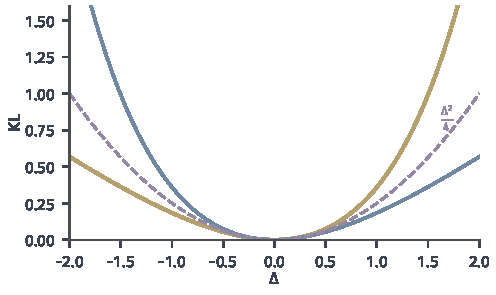
\includegraphics[width=84mm]{figures/07-probability/07-distribution-optimization/matplotlib/igeo-kl-quadratic/figure.pdf}
  \caption{对数方差坐标$\tau=\ln\sigma^{2}$中位移$\Delta$引起的KL散度。蓝线：$D_{\mathrm{KL}}(P_{\tau}\Vert P_{\tau+\Delta})=\frac12(\Delta+\mathrm{e}^{-\Delta}-1)$；黄线：反方向$\frac12(\mathrm{e}^{\Delta}-\Delta-1)$；紫色虚线：二次近似$\frac12G_{\tau\tau}\Delta^{2}=\Delta^{2}/4$。三条曲线在$\Delta=0$附近重合，远处分开。}
  \label{fig:igeo-kl-quadratic}
\end{BookInlineFigure}

局部非退化也推不出全局的参数唯一。在$\mathcal{N}(\theta^{2},1)$中取$\theta=1$，$G(1)=4>0$，二次近似说位移$\delta=-2$应带来约$\frac12\cdot4\cdot4=8$的KL散度；而$\theta+\delta=-1$与$\theta=1$给出同一个分布，真实的KL散度为零。展开只对足够小的$\bm{\delta}$成立，“足够小”有多小，取决于族在这一点附近的形状。

\paragraph{Fisher椭圆}
在二维参数空间中，位移的集合
\[
  \Bigl\{\bm{\delta}:\frac12\bm{\delta}^{\top}\bm{G}(\bm{\theta})\bm{\delta}=\varepsilon\Bigr\}
\]
放在$\bm{\theta}$处是一个以$\bm{\theta}$为中心的椭圆。局部看，椭圆上每个点代表的邻近分布与中心分布的KL散度都约为$\varepsilon$。高斯族在$(\mu,\sigma)$坐标下，由式~\eqref{eq:igeo-gauss-fisher}，椭圆沿$\mu$方向的半轴为$\sigma\sqrt{2\varepsilon}$，沿$\sigma$方向的半轴为$\sigma\sqrt{\varepsilon}$。

图~\ref{fig:igeo-fisher-ellipses}把这些椭圆画在$(\mu,\sigma)$半平面上。同一行的椭圆一样大：平移不改变局部尺度。越靠近$\sigma=0$，椭圆越小：分布越窄，参数只要稍动就造成同样大小的变化。每个椭圆横向比纵向宽$\sqrt2$倍：同样的KL预算下，均值可以比$\sigma$多动一些。把这些椭圆当作各点的“单位圆”，参数平面就带上了一把随位置变化的尺子。

\begin{BookInlineFigure}
  \centering
  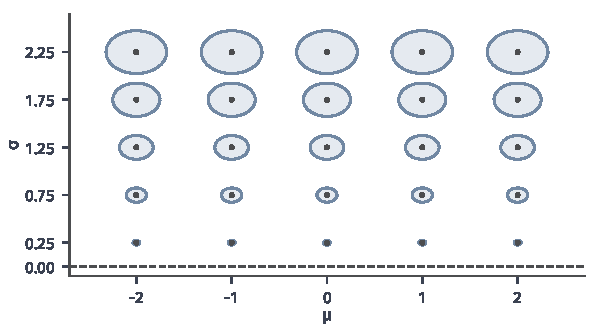
\includegraphics[width=100mm]{figures/07-probability/07-distribution-optimization/matplotlib/igeo-fisher-ellipses/figure.pdf}
  \caption{高斯族在$(\mu,\sigma)$半平面上的Fisher椭圆$\frac12\bm{\delta}^{\top}\bm{G}\bm{\delta}=0.01$。中心为深灰点，$\sigma$取$0.25,0.75,\dots,2.25$，$\mu$取$-2,\dots,2$；半轴为$0.141\sigma$（$\mu$方向）与$0.1\sigma$（$\sigma$方向）。深灰虚线$\sigma=0$不属于参数集合。}
  \label{fig:igeo-fisher-ellipses}
\end{BookInlineFigure}

\subsection{坐标变换}
\label{sec:igeo-coordinates}

同一个高斯族可以用$(\mu,\sigma)$、$(\mu,\sigma^{2})$、$(\mu,\ln\sigma^{2})$或第~\ref{chap:distribution-families}章的自然参数来编号。章首的例子已经显示，同样增加$0.1$，在方差坐标中引起的KL随起点变化，在对数方差坐标中则不变。分布族没有变，变的只是编号的方式。Fisher信息的数值随编号而变，这在章首已经看到；问题是它所表示的“局部变化有多大”是否也依赖于编号。

设$\Xi\subset\mathbb{R}^{k}$是开集，$\bm{\varphi}:\Xi\to\Theta$是连续可微的双射，其逆也连续可微，Jacobian矩阵
\[
  \bm{J}(\bm{\xi})=\frac{\partial\bm{\theta}}{\partial\bm{\xi}}\in\mathbb{R}^{k\times k},\qquad J_{i,j}=\frac{\partial\theta_{i}}{\partial\xi_{j}},
\]
处处非奇异。新坐标下的族是$q_{\bm{\xi}}=p_{\bm{\varphi}(\bm{\xi})}$。它仍是正则族：支撑不变，逐点可微由链式法则得到，而在$\bm{\xi}$的紧邻域上$\bm{J}$有界，原来的控制函数乘以这个界仍然可积。

\begin{theorem}[得分与Fisher信息的坐标变换]
\label{thm:igeo-reparam}
在上述设定下，记$\bm{\theta}=\bm{\varphi}(\bm{\xi})$，$\bm{J}=\bm{J}(\bm{\xi})$，则
\begin{equation}
  \bm{s}^{\Xi}_{\bm{\xi}}(x)=\bm{J}^{\top}\bm{s}_{\bm{\theta}}(x),\qquad
  \bm{G}^{\Xi}(\bm{\xi})=\bm{J}^{\top}\bm{G}(\bm{\theta})\bm{J}.
  \label{eq:igeo-reparam}
\end{equation}
对任意$\mathrm{d}\bm{\xi}\in\mathbb{R}^{k}$，令$\mathrm{d}\bm{\theta}=\bm{J}\,\mathrm{d}\bm{\xi}$，则
\begin{equation}
  \mathrm{d}\bm{\xi}^{\top}\bm{G}^{\Xi}(\bm{\xi})\,\mathrm{d}\bm{\xi}=\mathrm{d}\bm{\theta}^{\top}\bm{G}(\bm{\theta})\,\mathrm{d}\bm{\theta}.
  \label{eq:igeo-invariant-form}
\end{equation}
\end{theorem}

\begin{proof}
由链式法则，对每个$j$，
\[
  \frac{\partial}{\partial\xi_{j}}\ln p_{\bm{\varphi}(\bm{\xi})}(x)=\sum_{i=1}^{k}\frac{\partial\ln p_{\bm{\theta}}(x)}{\partial\theta_{i}}\,\frac{\partial\theta_{i}}{\partial\xi_{j}},
\]
写成向量就是式~\eqref{eq:igeo-reparam}的第一式。$\bm{J}$不随$x$变化，代入式~\eqref{eq:igeo-fisher}，
\[
  \bm{G}^{\Xi}(\bm{\xi})=\mathbb{E}\bigl[\bm{J}^{\top}\bm{s}_{\bm{\theta}}\bm{s}_{\bm{\theta}}^{\top}\bm{J}\bigr]=\bm{J}^{\top}\bm{G}(\bm{\theta})\bm{J}.
\]
最后，
\[
  \mathrm{d}\bm{\xi}^{\top}\bm{J}^{\top}\bm{G}(\bm{\theta})\bm{J}\,\mathrm{d}\bm{\xi}=(\bm{J}\,\mathrm{d}\bm{\xi})^{\top}\bm{G}(\bm{\theta})(\bm{J}\,\mathrm{d}\bm{\xi}),
\]
即式~\eqref{eq:igeo-invariant-form}。
\end{proof}

式~\eqref{eq:igeo-invariant-form}的含义是：$\mathrm{d}\bm{\xi}$与$\mathrm{d}\bm{\theta}=\bm{J}\,\mathrm{d}\bm{\xi}$是同一个无穷小位移在两套坐标中的分量。它们的数字不同，矩阵也不同，但二次型给出同一个值，而由定理~\ref{thm:igeo-kl-expansion}，这个值的一半正是该位移引起的局部KL。改变的是记录方式，不变的是分布本身的局部变化。

\paragraph{方差与对数方差}
在$\mathcal{N}(0,v)$中，$\ln p_{v}(x)=-\frac12\ln(2\pi v)-\frac{x^{2}}{2v}$，于是
\[
  s_{v}(x)=-\frac1{2v}+\frac{x^{2}}{2v^{2}}=\frac{x^{2}-v}{2v^{2}} .
\]
$X^{2}$的方差是$2v^{2}$，所以
\[
  G_{vv}=\frac{\operatorname{Var}(X^{2})}{4v^{4}}=\frac{2v^{2}}{4v^{4}}=\frac1{2v^{2}}.
\]
改用$\tau=\ln v$，$v=\mathrm{e}^{\tau}$，$J=\mathrm{d}v/\mathrm{d}\tau=v$，由式~\eqref{eq:igeo-reparam}，
\[
  G_{\tau\tau}=v^{2}\cdot\frac{1}{2v^{2}}=\frac12 ,
\]
与上一小节由KL展开读出的系数一致。

在$v=4$处取$\Delta v=0.4$，对应$\Delta\tau=\ln1.1\approx0.0953$，一阶近似为$0.1$。两套坐标下的二次型分别是
\[
  \frac12\cdot\frac1{32}\cdot0.4^{2}=0.0025,\qquad\frac12\cdot\frac12\cdot0.1^{2}=0.0025,
\]
完全相等；精确的KL为$0.0022$。而两个位移的欧氏长度一个是$0.4$，一个约是$0.1$。图~\ref{fig:igeo-coordinate-rulers}画出$v=0.5,1,2,4$四处局部KL不超过$0.01$的参数区间：在$v$轴上，区间长度与$v$成正比；在$\tau$轴上，四段一样长。

\begin{BookInlineFigure}
  \centering
  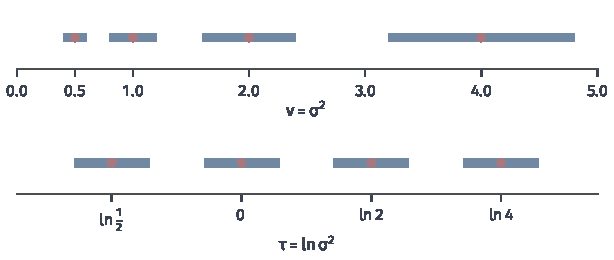
\includegraphics[width=104mm]{figures/07-probability/07-distribution-optimization/matplotlib/igeo-coordinate-rulers/figure.pdf}
  \caption{$\mathcal{N}(0,v)$在$v=0.5,1,2,4$（红点）处满足$\frac12G\,d^{2}\leq0.01$的参数区间（蓝色粗线）。上：方差坐标$v$，半长$0.2v$；下：对数方差坐标$\tau=\ln v$，半长都是$0.2$。两行对应的是同一组分布区间。}
  \label{fig:igeo-coordinate-rulers}
\end{BookInlineFigure}

\paragraph{二维的例子}
把均值加进来。在$(\mu,v)$坐标下，同样的计算给出
\[
  \bm{G}(\mu,v)=\begin{bmatrix}1/v&0\\0&1/(2v^{2})\end{bmatrix},\qquad
  \bm{G}(\mu,\tau)=\begin{bmatrix}1/v&0\\0&1/2\end{bmatrix}.
\]
在$\mathcal{N}(1,4)$处取$(\mu,\tau)$坐标中的位移$(0.6,\ 0.566)$，它满足$\frac12(0.25\cdot0.36+0.5\cdot0.32)=0.125$。换到$(\mu,v)$坐标，$\mathrm{d}v=v\,\mathrm{d}\tau$，位移变为$(0.6,\ 2.263)$，二次型为
\[
  \frac12\Bigl(\frac14\cdot0.36+\frac1{32}\cdot5.12\Bigr)=\frac12(0.09+0.16)=0.125 .
\]
图~\ref{fig:igeo-tangent-ellipses}中，绿色箭头在两张图里的分量相差约四倍，但箭头都恰好落在各自的椭圆$\frac12\bm{\delta}^{\top}\bm{G}\bm{\delta}=0.125$上。

\begin{BookInlineFigure}
  \centering
  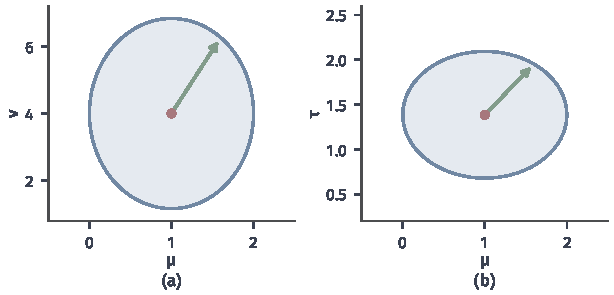
\includegraphics[width=104mm]{figures/07-probability/07-distribution-optimization/matplotlib/igeo-tangent-ellipses/figure.pdf}
  \caption{同一个位移在两套坐标中的表示，中心为$\mathcal{N}(1,4)$（红点）。(a)$(\mu,v)$坐标；(b)$(\mu,\tau)$坐标，$\tau=\ln v$。蓝色椭圆为$\frac12\bm{\delta}^{\top}\bm{G}\bm{\delta}=0.125$，绿色箭头分别是$(0.6,\,2.263)$与$(0.6,\,0.566)$，两者表示同一个位移，都落在椭圆上。两图纵轴的单位不同。}
  \label{fig:igeo-tangent-ellipses}
\end{BookInlineFigure}

\paragraph{几何的说法}
把每一种参数化看成分布族上的一张坐标卡，坐标之间的转换就是流形的坐标变换，无穷小位移就是切向量，它的分量按$\bm{J}$变换，这些概念可参考\BookChapterRef{chap:manifold-basics}{卷四第24章“流形的基本概念”}。式~\eqref{eq:igeo-invariant-form}说明，
\[
  \langle\bm{a},\bm{b}\rangle_{\bm{G}}=\bm{a}^{\top}\bm{G}(\bm{\theta})\bm{b}
\]
是切向量之间不依赖坐标的对称双线性形式。当$\bm{G}$处处正定且光滑变化时，它是参数流形上的一个Riemann度量，称为\term{Fisher度量}（Fisher metric），一般定义可参考\BookChapterRef{chap:riemannian-geometry}{卷四第27章“黎曼几何”}。

这个说法也标出了本节结论的边界。坐标变换下保持的是切向量的长度，即局部变化的大小；矩阵的元素、参数位移的欧氏长度都不保持。在$\bm{G}$退化的点，二次型只是半正定的，不能当作度量，需要先按第~\ref{sec:igeo-fisher}节的办法辨认退化的来源。
